\documentclass[letterpaper]{article}
\usepackage[letterpaper,top=1in,bottom=1in,left=1in,right=1in]{geometry}
\usepackage[utf8]{inputenc}
\usepackage{graphicx}
\usepackage[T1]{fontenc}
\usepackage{times}      % Loads the Times-Roman Fonts
\usepackage{mathptmx}   % Loads the Times-Roman Math Fonts
\usepackage{helvet}
\usepackage[sf,bf]{titlesec}
\usepackage{lineno}
\usepackage{setspace}
\usepackage[style=nejm]{biblatex}
\addbibresource{references.bib}
\usepackage{caption}
\captionsetup[figure]{labelfont={sf,bf}}

\setlength{\parindent}{0em}
\setlength{\parskip}{1em}

\begin{document}

\section*{Considering within-host diversity in phylogenetic analysis for detecting clusters of new HIV infections}

August Guang$^{1,2}$, Mark Howison$^3$, Charles Lawrence$^4$, Casey W. Dunn$^5$, Rami Kantor$^6$

$^1$ Center for Computational Biology of Human Disease, Brown University, Providence, RI, USA

$^2$ Center for Computation and Visualization, Brown University, Providence, RI, USA

$^3$ Research Improving People's Lives, Providence, RI, USA

$^4$ Division of Applied Mathematics, Brown University, Providence, RI, USA

$^5$ Department of Ecology and Evolutionary Biology, Yale University, New Haven, CT, USA

$^6$ Division of Infectious Diseases, The Alpert Medical School, Brown University, Providence, RI, USA

\doublespace
%\linenumbers
\section*{Abstract}

\textbf{Background:} Phylogenetic analysis of HIV sequences obtained as part of clinical care is increasingly applied to detect clustering of new HIV infections and inform public health interventions to disrupt transmission. Conventional approaches summarize the within-host HIV diversity with a single consensus sequence per individual of only the \emph{pol} gene, obtained from Sanger or next-generation sequencing (NGS).

\textbf{Methods:} We evaluate the robustness of the consensus approach and the potential benefits of considering the within-host diversity in phylogenetic analysis and cluster inference for all newly HIV-diagnosed individuals within six months at the largest HIV center in Rhode Island, USA, representing \~80\% of the state's HIV epidemic. We compare Sanger and NGS-derived \emph{pol} and near-whole genome consensus sequences to an alternate approach that samples many sequences per individual from a profile hidden Markov model of their NGS data.

\textbf{Results:} The space of phylogenies inferred through sampling is multi-modal, suggesting that a consensus-inferred phylogeny is not an appropriate summary of within-host variation. Cluster inference differs in phylogenies from consensus sequences from Sanger and NGS data, and across gene regions.

\textbf{Discussion:} The choice of sequencing and summarization methods affects the detection of clusters, and should be considered carefully in public health applications of phylogenetic analysis to disrupt HIV transmission.

\section*{Background}

Public health officials and providers are generally interested in inferring transmission links between individuals with HIV to inform and improve HIV treatment and prevention. In the absence of reliable patient contact histories, phylogenetic analysis of viral sequence data can and has been be used to infer transmission clusters \parencite{leitner}, under the assumption that two individuals sharing a most recent common ancestor in a phylogeny are more likely to share a transmission link in the real, unobservable transmission network. The application of phylogenetic analysis and cluster inference techniques in public health interventions to disrupt transmission was delineated as one of the four key pillars for achieving the Department of Health and Human Services' recently-announced plan for ending the HIV epidemic in the US \parencite{fauci}.

While historically the phylogenetic informativeness of the \emph{pol} region of the HIV genome was suggested and contested \parencite{hue, sturmer}, its use is now widespread in phylogenetic analysis and cluster inference, often due to the availability of \emph{pol} sequences from guideline-recommended routine clinical drug resistance testing by commercial Sanger sequencing \parencite{dhhs}. In a recent review of HIV cluster inference, 98 out of 105 (93\%) analyzed the \emph{pol} region \parencite{hassan}.

The increasing availability of NGS technology has led to longer and deeper sequencing of HIV, and data sets more routinely cover nearly the whole genome with thousands or more reads at each site \parencite{voelkerding}. Recent evidence suggests improvements in both phylogenetic analysis and cluster inference from near-whole genome HIV sequences obtained with NGS. For example, Yebra \emph{et al.} \parencite{yebra} found that the accuracy of phylogenetic reconstruction and cluster inference on simulated sequences improved with longer genomic regions (with the best accuracy from a \emph{gag}-\emph{pol}-\emph{env} concatenation). Novitsky \emph{et al.} \parencite{novitsky} similarly studied the effects on cluster inference of using longer genomic regions from real near-whole genome Sanger sequences, and found that the proportion of sequences in clusters increased with longer sequence regions.

While the potential advantages of longer sequences in inferring transmission have been demonstrated, the advantages of deeper sequencing have not yet been fully investigated, and whether it can improve HIV molecular clustering inference is unknown. In part this is because researchers often rely on consensus sequences that discard all but the majority variant at each site, since most phylogenetic methods require a single fully resolved sequence for each individual included in the phylogeny. Accordingly, researchers studying HIV transmission summarize the within-host HIV variation present in NGS data sets with a consensus sequence. In the larger context of phylogenetic methods (e.g. beyond their application to HIV sequences), this consensus approach carries an underlying statistical assumption of \emph{low relative entropy} \parencite{guang}. In the context of HIV, this assumption is that a consensus sequence can adequately capture all of the relevant information about within-host variation available in a deeply-sequenced NGS data set. Some previous studies of HIV transmission dynamics have accounted for this variation with coalescent within-host evolutionary models \parencite{giardina, romero-severson}, but such models still assume a consensus sequence as the observed data.

In this study, we examine how well the assumption underlying the consensus approach holds on a NGS data set comprising all newly HIV-diagnosed individuals during a six month time period from the largest HIV center in Rhode Island, USA, representing \~80\% of the state's HIV epidemic. We present a new approach called \emph{profile sampling} that uses the within-host variation in the NGS data to assess the robustness of the consensus approach for phylogenetic analysis and cluster inference.

\section*{Methods}

\subsection*{Data collection and sequencing}

HIV-1 \emph{pol} sequences (HXB2 positions ) available for clinical care were collected from the 37 individuals newly diagnosed with HIV during the first half of 2013 and treated at The Miriam Hospital Immunology Center in Providence, Rhode Island, USA. Inclusion criteria were: (i) adults with HIV, 18 years of age or older; (ii) diagnosed with HIV during the first six months of 2013; and (iii) available \emph{pol} sequence from routine drug resistance testing. Patient identifiers were removed and all analysis was conducted with de-identified sequence data.

Blood specimens were obtained from participants with their consent and processed to isolate peripheral blood mononuclear cells (PMBC) and plasma. Using both Sanger and NGS, near-whole genome viral sequences were obtained from one of those compartments; plasma for participants with detectable viral load and PBMC for participants with undetectable viral load or unsuccessful plasma genotyping. Total nucleic acids were extracted for genotyping and an in-house genotyping assay was used to generate the near-whole genome based on previously published methods \parencite{nadai, di_giallonardo}. For each sample, two cDNA templates were generated by SuperscriptIII First Strand Synthesis System (Thermofisher, Carlsbad, CA), followed by eight separate nested PCR reactions; these eight amplicons span the near-whole genome of HIV.  Final amplicon products were sequenced by the Sanger method using 3100 Genetic Analyzer (Applied Biosystems, Foster City, CA) and sequenced by NGS using Nextera XT DNA Library Prep chemistry (Illumina, San Diego, CA) to generate multiplexed libraries for Illumina's MiSeq platform with 250 base paired-end reads. Sanger consensus sequences were generated manually using Sequencher version 5.2.4 (Gene Codes, Ann Arbor, MI) to confirm degenerate nucleotides. NGS data were processed and demultiplexed using BaseSpace cloud based application? (Illumina, San Diego, CA).

\subsection*{Profile sampling}

We introduce a new approach for incorporating within-host variation into phylogentic analysis, called \emph{profile sampling}. We start by aligning each individual's NGS reads using the hivmmer pipeline \parencite{howison}, which we extended to support near-whole genome HIV data and to perform codon-aware alignment within each gene (pending release as hivmmer version 0.3.0). A key feature of this pipeline is its use of profile hidden Markov models (HMMs) to model and align collections of HIV sequences. Profile HMMs have been used in many kinds of biological sequence analyses and are particularly well-suited to modeling variation in populations of sequences \parencite{eddy2004}. Briefly, hivmmer performs quality control and error correction in overlapping regions of the read pairs using PEAR version 0.9.11 \parencite{zhang}, translates them into each possible reading frame, aligns them in amino acid space to profile HMMs of all group M reference sequences from the Los Alamos National Lab HIV Database \parencite{losalamos} with the profile HMM alignment tool HMMER version 3.1b2 \parencite{eddy2013}, and produces a codon frequency table across the near-whole HIV genome. We refer to this resulting codon frequency table as the individual's HIV \emph{profile}.

For each patient, we construct a population of fully-resolved sequences by sampling codons at each site in the genome using the codon frequencies from the profile. The collection of sampled sequences captures the empirical distribution of within-host variation at the codon level. We sample 500 sequences from each individual's profile, then collate the sampled sequences into 500 profile-sampled data sets, each having one sampled sequence per individual. We construct the 500 fully-resolved sequences in order to use existing phylogenetic methods, because there is currently no published method to our knowledge for inferring a phylogeny directly from the proflie representation of the individual's within-host variation.

We perform phylogenetic inference on each of the 500 profile-sampled data sets by estimating a multiple sequence alignment with mafft version 7.313 \parencite{katoh} and a maximum-likelihood phylogeny with the GTRCAT model and 100 rapid bootstrap replicates using RAxML version 8.2.12 \parencite{stamatakis}. In addition to the 500 profile-sampled phylogenies, we infer two additional phylogenies from the NGS consensus sequences and Sanger consensus sequences with the same tools and parameters. We perform cluster inference on these phylogenies using Cluster Picker \parencite{ragonnet-cronin} with thresholds of 80\% bootstrap support and 4.5\% genetic distance. Analysis source code is available from \url{https://github.com/kantorlab/hiv-profile-sampling}.

In addition to performing these analyses on the near-whole genome sequences (``wgs''), we also perform them on subsets of the sequences in three clinically relevant regions: the protease and reverse transcriptase regions at the beginning of the \emph{pol} gene (``prrt''), the \emph{int} gene, and the \emph{env} gene. The prrt region and \emph{int} are routinely sequenced in clinical care to detect drug resistance mutations and inform clinical choices of anti-retroviral therapy. The \emph{env} region is sequenced to genotypically infer viral tropism and co-receptor usage.

\section*{Results}

\subsection*{Profile sampling estimates within-host diversity}

We estimate the within-host diversity for individuals as the average percent difference across all pairwise comparisons of their 500 profile-sampled nucleotide sequences. Variation in within-host diversity could be due to a variety of biological factors, such as virus mutation rate, effective viral population size, and time since infection, as well as technical factors such as sequencing depth and sequencing error rates. These pairwise differences are calculated using the Hamming distance \parencite{allam} (which is also called the $p$-distance in the literature on HIV genetic diversity \parencite{maldarelli, hassan}). Figure 1 shows the estimated within-host percent diversity in each examined genomic region across individuals, ordered by \emph{env}, which we expected \emph{a priori} to be the most variable region. The largest estimated diversity is in \emph{env} for individual MC28 (4.0\%), and \emph{env} has the overall largest range in estimated diversity (0.2\% to 4.0\%). The other regions have ranges of 0.2\% to 1.9\% (prrt), 0.1\% to 2.0\% (\emph{int}) and 0.2\% to 2.6\% (wgs). These ranges are comparable to prior studies on within-host diversity \parencite{li, zanini}. These estimates of within-host diversity from the HIV profiles suggest that the consensus approach is discarding potentially-relevant information that is present in the NGS data.

\subsection*{Phylogenetic estimates are sensitive to within-host diversity}

Next, we investigate the impact of within-host diversity on phylogenetic topology and evolutionary distance estimates. To examine the variation in topology, we calculate the pairwise geodesic distance \parencite{billera,owen} among the 500 phylogenies from the profile samples, as well as the phylogenies from the NGS and Sanger consensus sequences. Then we perform multi-dimensional scaling (MDS) on the resulting distance matrix to visualize the topological space in two dimensions (Figure 2). The results show that the topological space is multi-modal, and the consensus phylogenies inferred from the consensus sequences do not fully summarize the clustering that occurs in topological space. The prrt region displays four topological clusters, and the NGS and Sanger consensus phylogenies are located in different clusters. There are two clusters in \emph{int}, and the phylogeny of NGS consensus sequences lies at the center of one of the clusters, while the phylogeny of Sanger consensus sequences is an outlier. The phlyogenies based on consensus sequences lie at opposite ends of the primary MDS axis in \emph{env}, and of the secondary MDS axis in the wgs region.

To examine the variation in estimated evolutionary distance, we sum the branch lengths within each phylogeny across all branches and across only the tip branches. We visualize the distribution of these branch length sums in Figure 3. Overall, the estimates are larger in \emph{env} and the wgs region, and smaller when restricting to only the tip branches. In some cases, the consensus phylogenies provide an adequate summary of the distribution (as in phylogeny of Sanger consensus sequences for all branches in \emph{env}, or the phylogeny of NGS consensus sequences for tip branches in \emph{env}). In other cases, the consensus phylogenies have estimates that are outliers in the distribution (as in both consensus phylogenies for either all or tip branches in the prrt region).

Taken together, the heterogeneity between the phylogenetic results from the profile sampling and the point estimates from the phylogenies of consensus sequences demonstrate that within-host virus sequence diversity impacts the inference of virus phylogeny across patients, and that the consensus approach for collapsing within-host sequence variation can obscure both the magnitude and effect of these impacts. For example, the variation can result in multi-modal phylogenetic results and the point estimates from the phylogenies of consensus sequences can be outliers.

\subsection*{Inferred clusters differ by sequencing method and genomic region}

Finally, we examine the clusters that are detected in phylogenies of NGS consensus sequences versus Sanger consensus sequences, and across the four genomic regions. The phylogeny of NGS consensus sequences detected eight clusters in prrt, nine in \emph{int}, four in \emph{env}, and six in wgs. Each cluster appears as a colored bar in the phylograms in Figure 4. We use the proportion of times a cluster appears across the 500 profile-sampled phylogenies as a measure of support for that cluster, and report it next to the colored bar. Some clusters are robustly detected across all regions, such as the cluster (MC25, MC26, MC52), which has support between 98\% and 100\%. Other clusters are detected at lower support, and are not detected consistently across regions. For example, cluster (MC14, MC59) only appears in the \emph{int} and wgs phylogenies, and at 60\% to 62\% support.  

The phylogeny of Sanger consensus sequences detects eight clusters in prrt, seven in \emph{int}, six in \emph{env}, and seven in wgs (Figure 5). As with the phylogeny of NGS consensus sequences, the support and consistency of cluster detection varies across regions. Cluster detection is mostly consistent with the NGS consensus, except for the cluster (MC17, MC21), which only occurs in \emph{env} in the Sanger consensus, and has zero support from the profile samples. Three clusters are consistently detected across NGS and Sanger, and across all regions: (MC23, MC24); (MC25, MC26, MC52); and (MC27, MC28).

\section*{Discussion}

The deeper sequencing provided by NGS captures within-host diversity far more effectively than previous generations of data acquisition methods. Though the first step in many NGS studies, to collapse this diversity into a single consensus sequence simplifies downstream analyses, results presented here demonstrate that it discards potentially interesting biological results and can mislead downstream analyses, as if the consensus may not be a good representative of the total population of sequences. These data could have epidemiological consequences as, for example, HIV molecular clustering can trigger public health activities to inform and improve HIV prevention and treatment interventions \parencite{peters}. As data acquisition increasingly shifts to NGS approaches, it is important to compare new results to the Sanger \emph{pol} consensus sequences that have been used since the first molecular characterizations of HIV sequence diversity.

Our analyses of Sanger \emph{pol} consensus sequences identifies 8 clusters; however, only 3 of the 8 are robustly detected across regions and in both NGS and Sanger consensus sequences.  In our comparison of cluster inference across genomic regions, we found that fewer clusters were detected overall in \emph{env} and wgs compared to prrt and \emph{int}. Prior studies of clustering from Sanger consensus sequences present mixed results on the prevalence of clustering across regions. Some studies have found concordant clustering across \emph{gag}-\emph{env} \parencite{han} and \emph{gag}-\emph{pol}-\emph{env} \parencite{english,kaye}, while others found fewer clusters in \emph{pol} than in \emph{env} \parencite{kapaata}, or fewer clusters in \emph{gag}-\emph{env} than in \emph{pol} \parencite{ndiaye}. The additional information available in NGS data, along with the cluster support measures provided by profile sampling, may help resolve these differences. In our results, for example, the cluster support measure establishes four clusters with robust support ($\geq$95\%) in only prrt and \emph{int}: (MC37, MC53); (MC17, MC20, MC21); (MC41, MC47, MC56); and (MC45, MC58).

Our approach presented here allows for the consideration of within-host variation using standard-off the shelf tools, just by propagating variation further in the analyses. Rather than collapse variation into consensus sequences prior to phylogenetic analysis, we create a profile that captures that variation, perform multiple phylogenetic analyses on sequences drawn from this profile, and then summarize the phylogenetic analyses. XXX  Future tools could incorporate the uncertainty directly into the phylogenetic inference process.

A limitation of our study is the small number of participants and the short time-frame patients were enrolled in. The participants have a dense temporal sampling, and comprise all newly HIV-diagnosed individuals in a six month period at the largest HIV center in Rhode Island, USA, who met the inclusion criteria. The overall size of the HIV epidemic in Rhode Island is much larger, estimated as 2,396 individuals in 2016 \parencite{ridoh}, but NGS data for this population are not currently available beyond those presented in this study. In future work, however, we hope to apply the profile sampling method to larger NGS data sets, to assess if cluster inference from Sanger versus NGS data agrees or differs especially for clusters larger than three individuals, which was the largest cluster size in this study.

Our construction of HIV profiles from NGS data is also limited by the accuracy of the NGS assays themselves. The codon frequencies in the profiles may be biased measures of the true within-host diversity because of biases in PCR amplification during sample preparation. Sequencing protocols such as Primer ID \parencite{jabara} have been introduced to reduce and correct for these biases. Unfortunately, the Primer ID protocol supports only a limited region of the HIV genome, and has not yet been extended to support near-whole genome sequencing of HIV, but future work could study this limited region to determine if cluster inference changes with the implementation of a Primer ID protocol.

In conclusion, the true HIV transmission network is unknown, but phylogenetic analysis and cluster inference are promising tools for aiding clinicians and public health officials \parencite{fauci}. Current phylogenetic approaches do not fully utilize the information on within-host diversity available in near-whole genome NGS data. As NGS data sets are increasingly available and become more representative of the current HIV epidemic, we suggest that the additional information they measure has the potential to improve the robustness of cluster inference.

\section*{Acknowledgments}

Mia Coetzer, Lauren Ledingham, Matt D'Antuono, Philip A. Chan

R01AI136058, K24AI134359, P30AI042853, Brown University DEANs Award.

\printbibliography

\begin{figure}[p!]
	\caption{Intra-patient genetic diversity (defined as the average percent difference across all pairwise comparisons of the 500 profile-sampled nucleotide sequences for a patient) is highest in \emph{env} for most individuals, and lies within the range of previously reported values.}
	\centering
	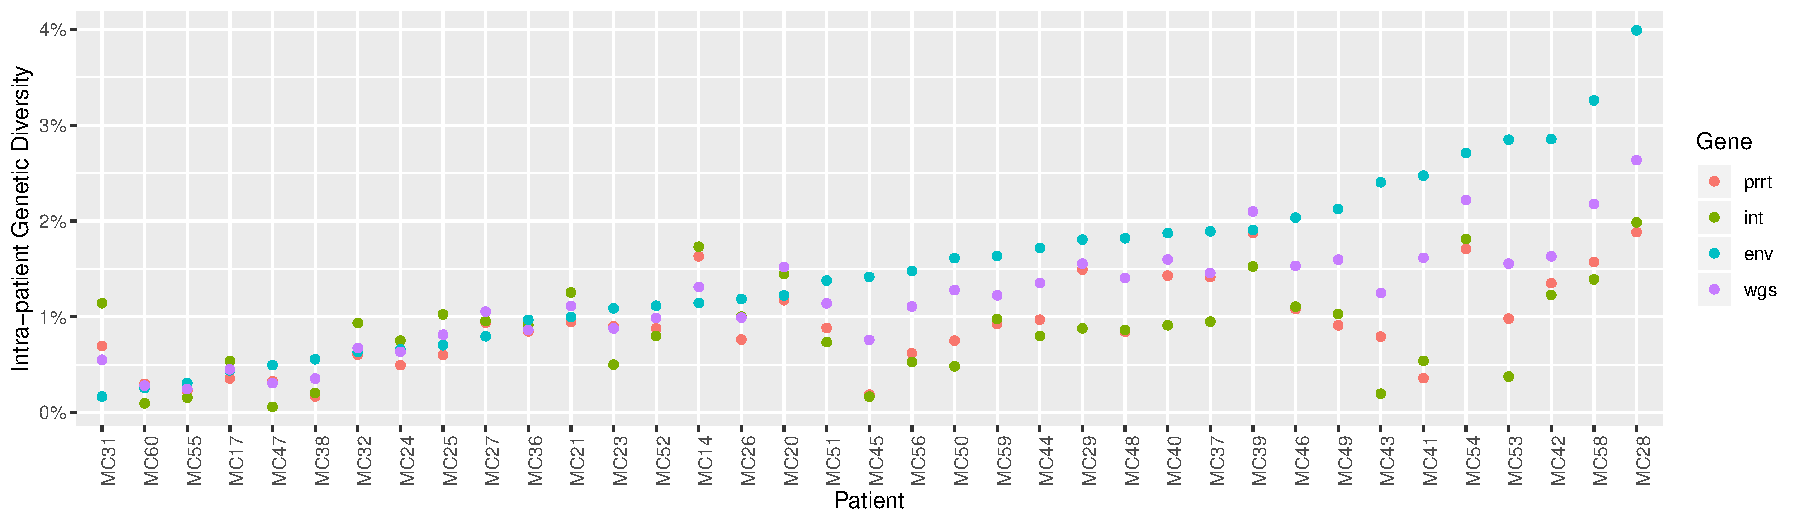
\includegraphics[width=\linewidth]{Figure1}
	\label{fig1}
\end{figure}

\begin{figure}[p!]
	\caption{Multi-dimensional scaling of pairwise geodesic distance among maximum-likelihood phylogenies from the profile-sampling approach show that the space of phylogenies inferred for the prrt and int regions are multi-modal. The phylogenies from consensus sequences (black dots) are point estimates that do not capture the full variation in phylogenies that can be inferred from deeply-sequenced NGS data.}
	\centering
	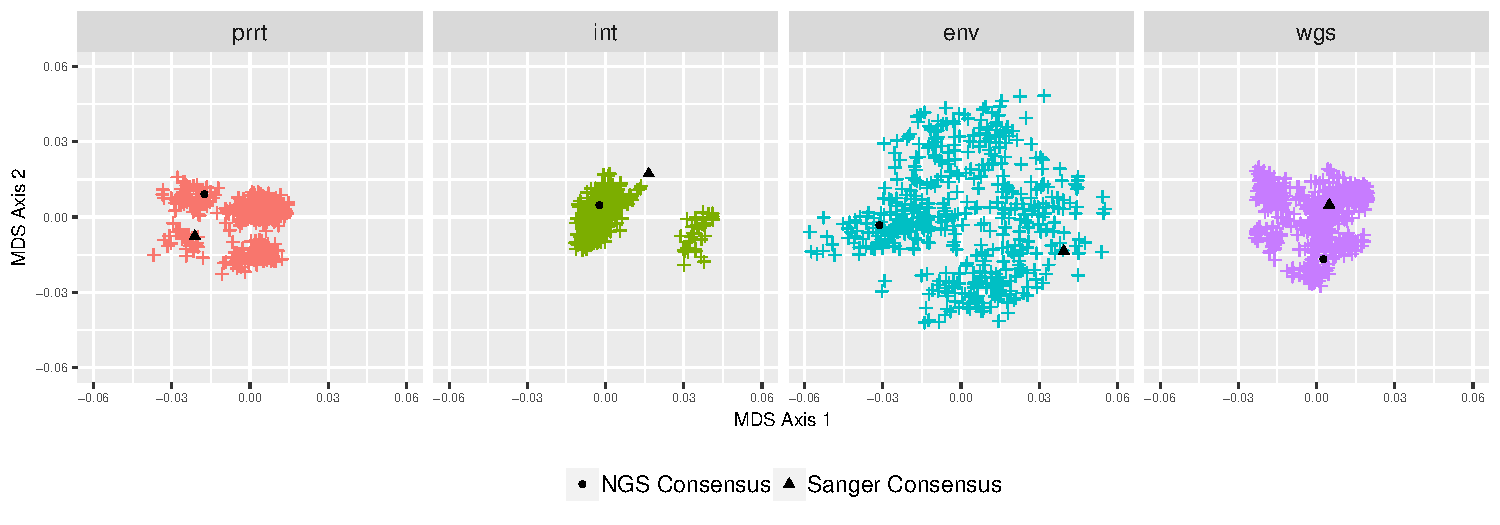
\includegraphics[width=\linewidth]{Figure2}
	\label{fig2}
\end{figure}
	
\begin{figure}[p!]
	\caption{The total branch length in each of the profile-sampled phylogenies also varies. The phylogenies from consensus sequences (black dots) can lie at extreme values within these distribution, both when considering the lengths across all branches and the lengths across only the branches at the tips.}
	\centering
	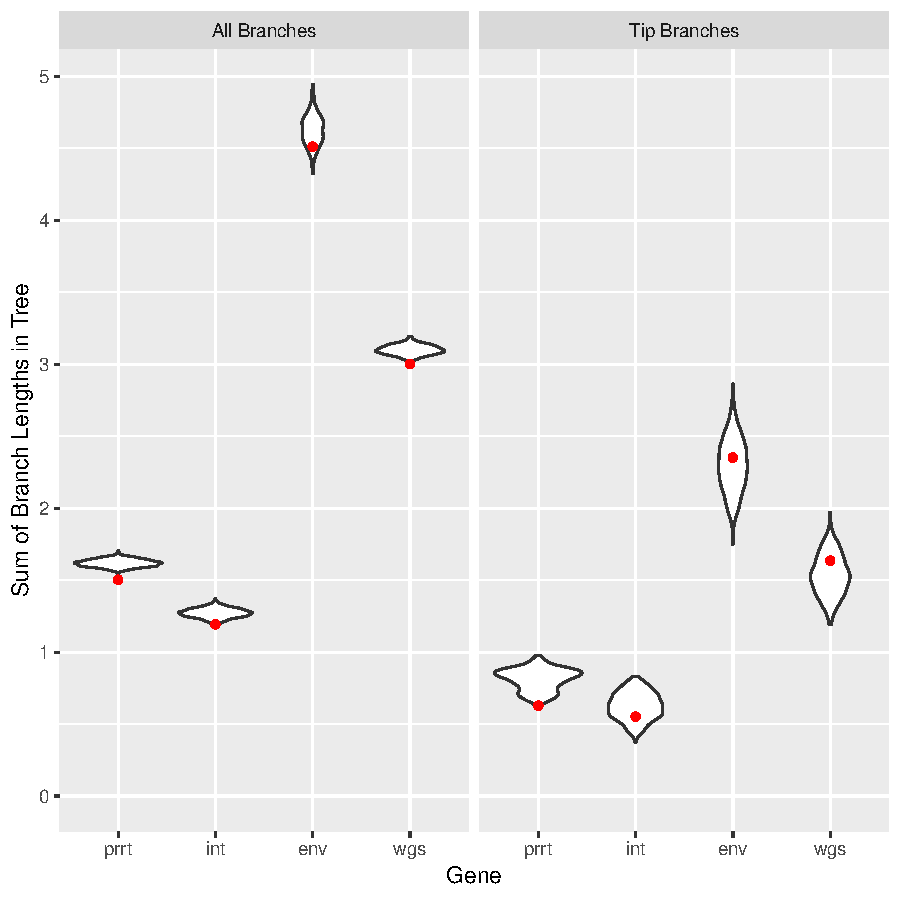
\includegraphics[width=3.25in]{Figure3}
	\label{fig3}
\end{figure}

\begin{figure}[p!]
	\caption{Clusters (vertical colored bars) inferred from the phylogenies of NGS consensus sequences differ across genomic regions. The largest number of clusters was inferred from the int region, and the smallest number from the env region. Profile sampling provides a bootstrapped measure of cluster support (annotation to bars).}
	\centering
	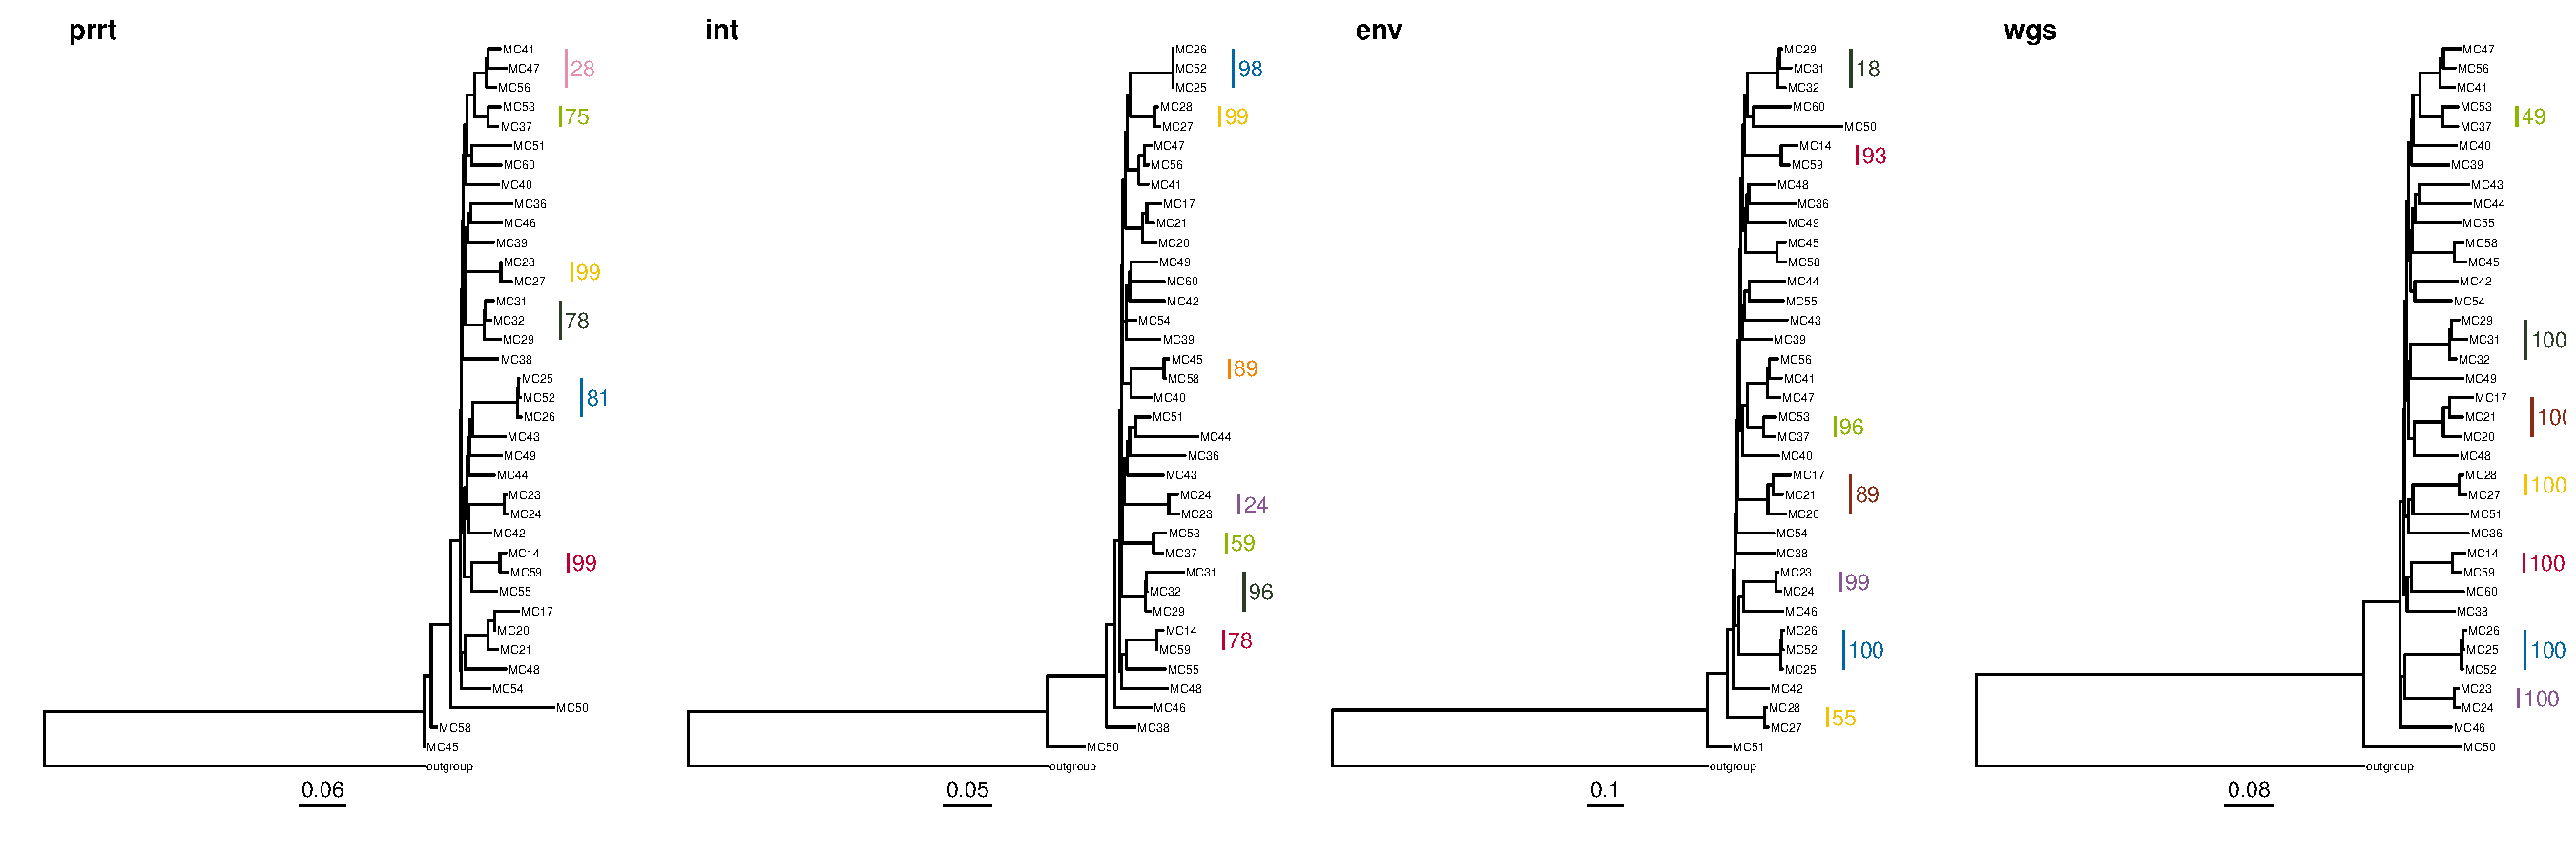
\includegraphics[width=\linewidth]{Figure4}
	\label{fig4}
\end{figure}

\begin{figure}[p!]
	\caption{Clusters (vertical colored bars) inferred from the phylogenies of Sanger consensus sequences differ across genomic regions. The largest number of clusters was inferred from the int region, and the smallest number from the env region. Profile sampling provides a bootstrapped measure of cluster support (annotation to bars).}
	\centering
	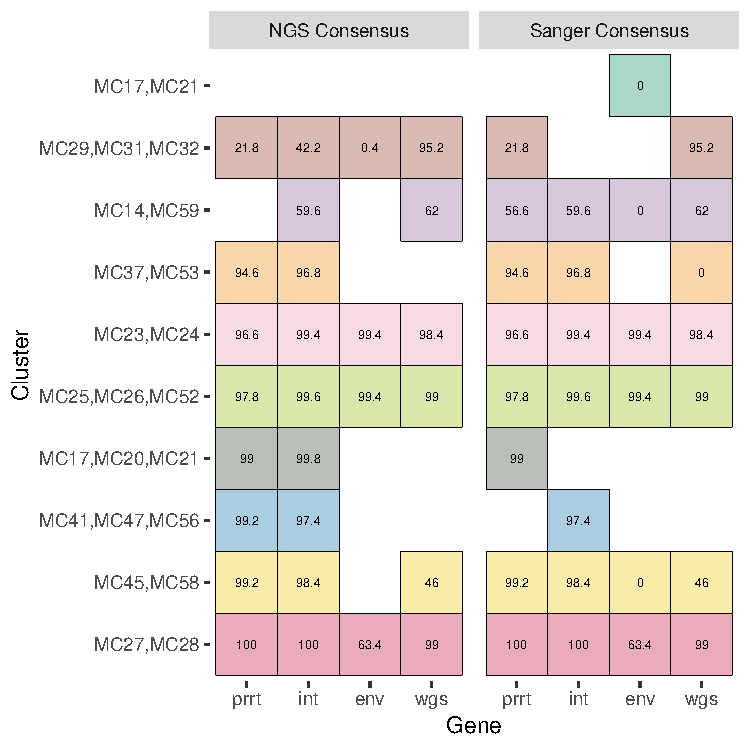
\includegraphics[width=\linewidth]{Figure5}
	\label{fig5}
\end{figure}

\newpage

\begin{figure}[p!]
	\caption{Summary of clusters identified by Sanger versus NGS consensus sequences across genomic regions. Numeric values indicate bootstrapped cluster support from the profile sampling method. A blank cell indicates that the cluster was not detected in that consensus sequence and genomic region.}
	\centering
	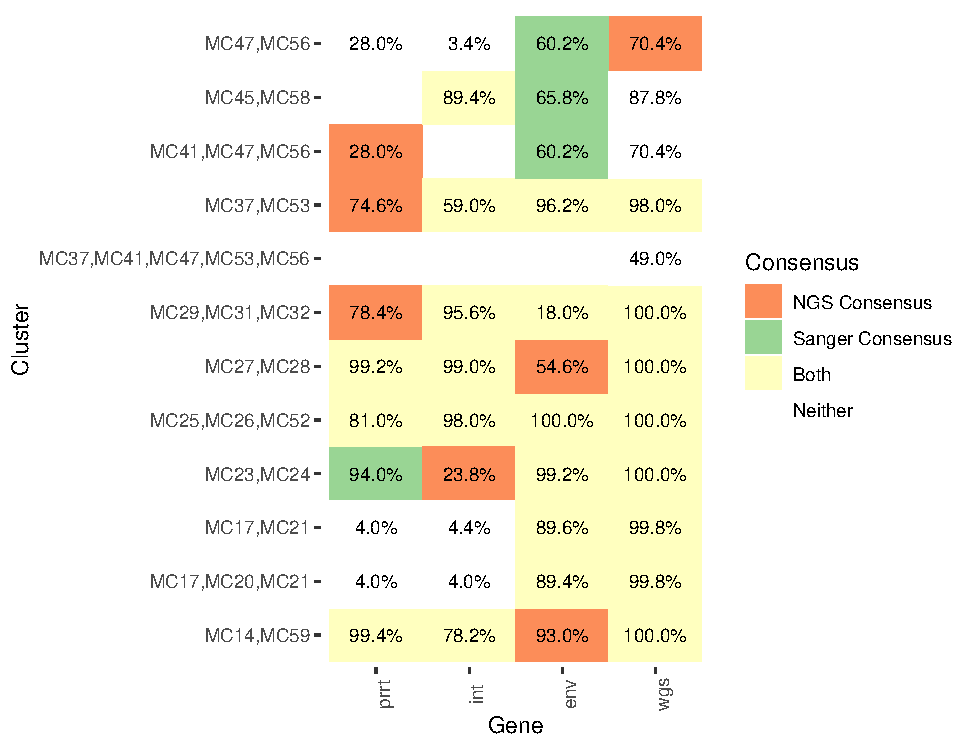
\includegraphics[width=3.25in]{Figure6}
	\label{fig6}
\end{figure}

\end{document}
